% Created by tikzDevice version 0.10.1 on 2016-04-02 13:30:33
% !TEX encoding = UTF-8 Unicode
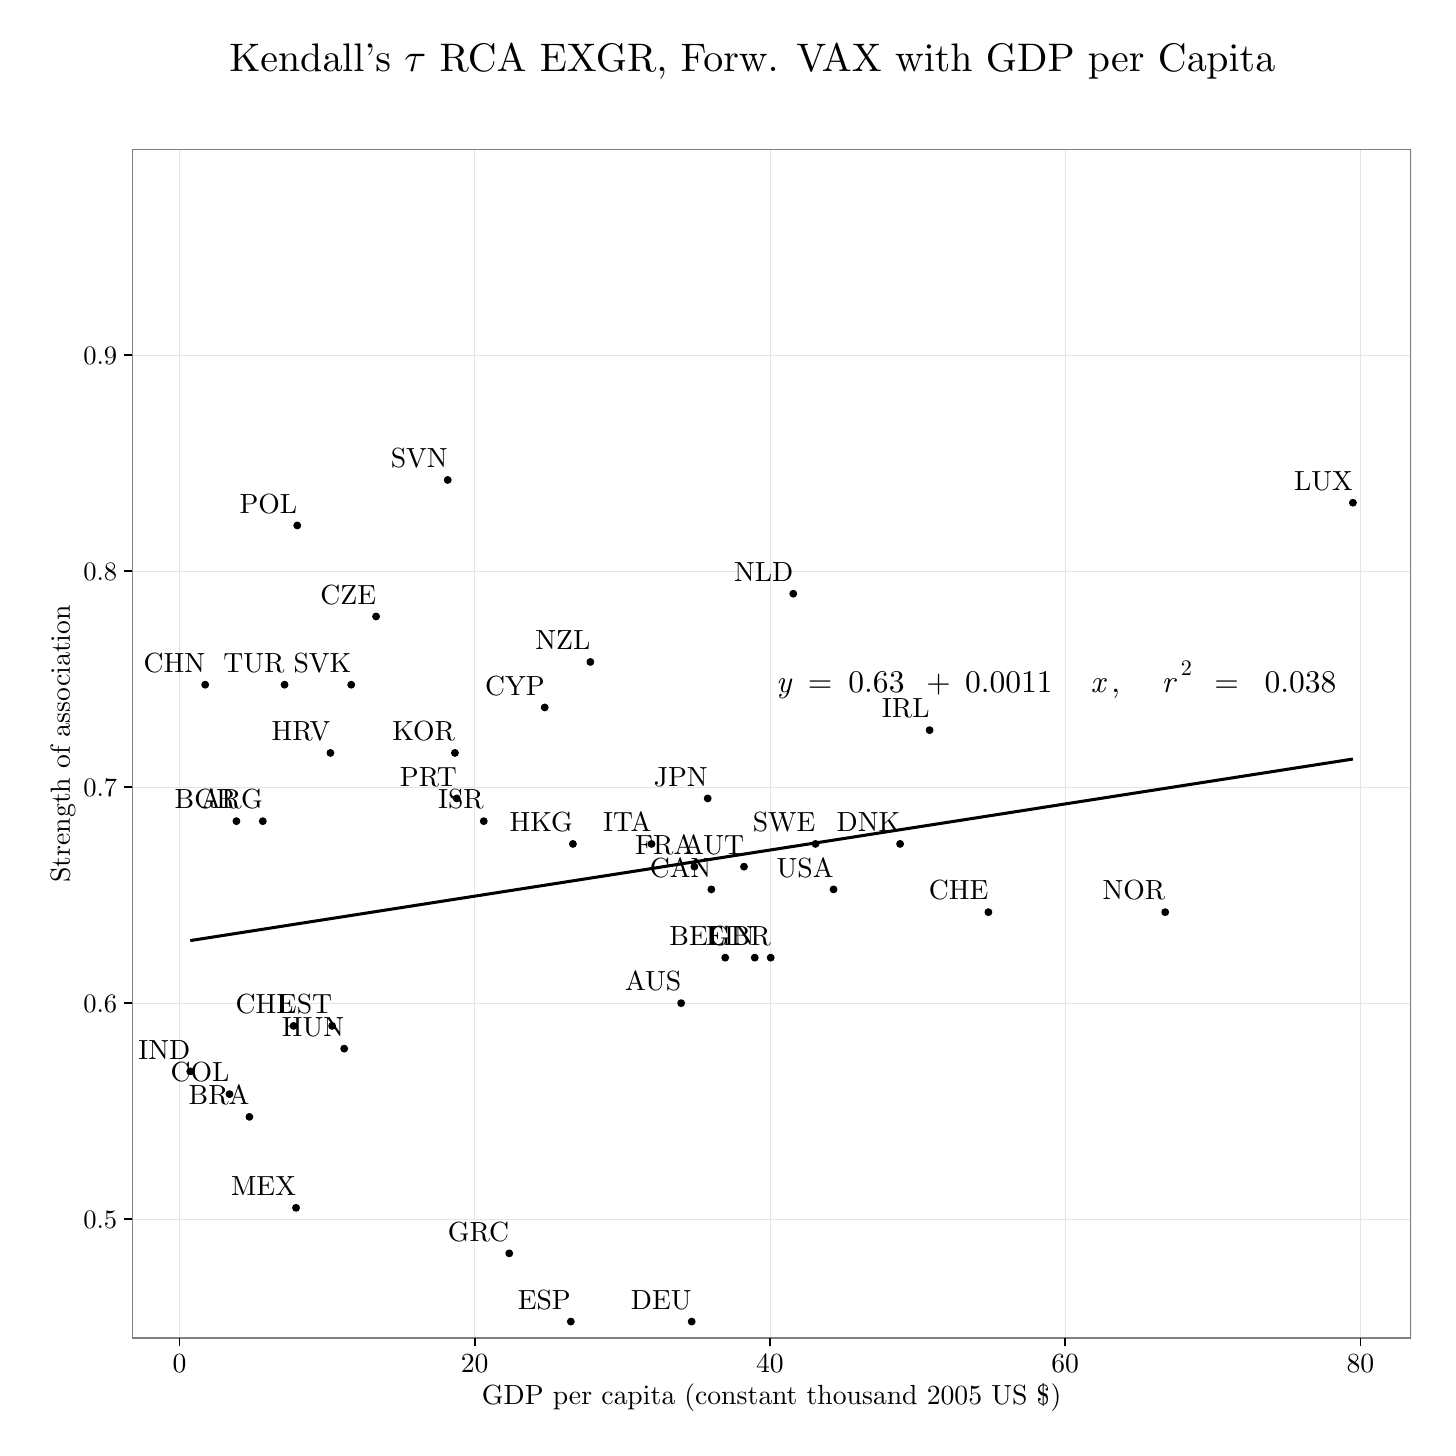
\begin{tikzpicture}[x=1pt,y=1pt]
\definecolor{fillColor}{RGB}{255,255,255}
\path[use as bounding box,fill=fillColor,fill opacity=0.00] (0,0) rectangle (505.89,505.89);
\begin{scope}
\path[clip] (  0.00,  0.00) rectangle (505.89,505.89);
\definecolor{drawColor}{RGB}{255,255,255}
\definecolor{fillColor}{RGB}{255,255,255}

\path[draw=drawColor,line width= 0.6pt,line join=round,line cap=round,fill=fillColor] (  0.00,  0.00) rectangle (505.89,505.89);
\end{scope}
\begin{scope}
\path[clip] ( 37.75, 32.37) rectangle (499.89,461.83);
\definecolor{fillColor}{RGB}{255,255,255}

\path[fill=fillColor] ( 37.75, 32.37) rectangle (499.89,461.83);
\definecolor{drawColor}{gray}{0.90}

\path[draw=drawColor,line width= 0.2pt,line join=round] ( 37.75, 75.32) --
	(499.89, 75.32);

\path[draw=drawColor,line width= 0.2pt,line join=round] ( 37.75,153.40) --
	(499.89,153.40);

\path[draw=drawColor,line width= 0.2pt,line join=round] ( 37.75,231.49) --
	(499.89,231.49);

\path[draw=drawColor,line width= 0.2pt,line join=round] ( 37.75,309.57) --
	(499.89,309.57);

\path[draw=drawColor,line width= 0.2pt,line join=round] ( 37.75,387.65) --
	(499.89,387.65);

\path[draw=drawColor,line width= 0.2pt,line join=round] ( 54.87, 32.37) --
	( 54.87,461.83);

\path[draw=drawColor,line width= 0.2pt,line join=round] (161.55, 32.37) --
	(161.55,461.83);

\path[draw=drawColor,line width= 0.2pt,line join=round] (268.23, 32.37) --
	(268.23,461.83);

\path[draw=drawColor,line width= 0.2pt,line join=round] (374.90, 32.37) --
	(374.90,461.83);

\path[draw=drawColor,line width= 0.2pt,line join=round] (481.58, 32.37) --
	(481.58,461.83);
\definecolor{drawColor}{RGB}{0,0,0}
\definecolor{fillColor}{RGB}{0,0,0}

\path[draw=drawColor,line width= 0.4pt,line join=round,line cap=round,fill=fillColor] ( 84.96,219.16) circle (  1.21);

\path[draw=drawColor,line width= 0.4pt,line join=round,line cap=round,fill=fillColor] (236.13,153.40) circle (  1.21);

\path[draw=drawColor,line width= 0.4pt,line join=round,line cap=round,fill=fillColor] (258.85,202.72) circle (  1.21);

\path[draw=drawColor,line width= 0.4pt,line join=round,line cap=round,fill=fillColor] (252.05,169.84) circle (  1.21);

\path[draw=drawColor,line width= 0.4pt,line join=round,line cap=round,fill=fillColor] ( 75.42,219.16) circle (  1.21);

\path[draw=drawColor,line width= 0.4pt,line join=round,line cap=round,fill=fillColor] ( 80.12,112.31) circle (  1.21);

\path[draw=drawColor,line width= 0.4pt,line join=round,line cap=round,fill=fillColor] (247.04,194.50) circle (  1.21);

\path[draw=drawColor,line width= 0.4pt,line join=round,line cap=round,fill=fillColor] (347.15,186.28) circle (  1.21);

\path[draw=drawColor,line width= 0.4pt,line join=round,line cap=round,fill=fillColor] ( 96.09,145.18) circle (  1.21);

\path[draw=drawColor,line width= 0.4pt,line join=round,line cap=round,fill=fillColor] ( 64.15,268.47) circle (  1.21);

\path[draw=drawColor,line width= 0.4pt,line join=round,line cap=round,fill=fillColor] ( 72.93,120.53) circle (  1.21);

\path[draw=drawColor,line width= 0.4pt,line join=round,line cap=round,fill=fillColor] (186.82,260.25) circle (  1.21);

\path[draw=drawColor,line width= 0.4pt,line join=round,line cap=round,fill=fillColor] (125.90,293.13) circle (  1.21);

\path[draw=drawColor,line width= 0.4pt,line join=round,line cap=round,fill=fillColor] (239.94, 38.33) circle (  1.21);

\path[draw=drawColor,line width= 0.4pt,line join=round,line cap=round,fill=fillColor] (315.25,210.94) circle (  1.21);

\path[draw=drawColor,line width= 0.4pt,line join=round,line cap=round,fill=fillColor] (196.27, 38.33) circle (  1.21);

\path[draw=drawColor,line width= 0.4pt,line join=round,line cap=round,fill=fillColor] (110.01,145.18) circle (  1.21);

\path[draw=drawColor,line width= 0.4pt,line join=round,line cap=round,fill=fillColor] (262.73,169.84) circle (  1.21);

\path[draw=drawColor,line width= 0.4pt,line join=round,line cap=round,fill=fillColor] (240.91,202.72) circle (  1.21);

\path[draw=drawColor,line width= 0.4pt,line join=round,line cap=round,fill=fillColor] (268.48,169.84) circle (  1.21);

\path[draw=drawColor,line width= 0.4pt,line join=round,line cap=round,fill=fillColor] (174.01, 62.99) circle (  1.21);

\path[draw=drawColor,line width= 0.4pt,line join=round,line cap=round,fill=fillColor] (197.02,210.94) circle (  1.21);

\path[draw=drawColor,line width= 0.4pt,line join=round,line cap=round,fill=fillColor] (109.40,243.82) circle (  1.21);

\path[draw=drawColor,line width= 0.4pt,line join=round,line cap=round,fill=fillColor] (114.37,136.96) circle (  1.21);

\path[draw=drawColor,line width= 0.4pt,line join=round,line cap=round,fill=fillColor] ( 58.76,128.75) circle (  1.21);

\path[draw=drawColor,line width= 0.4pt,line join=round,line cap=round,fill=fillColor] (325.91,252.04) circle (  1.21);

\path[draw=drawColor,line width= 0.4pt,line join=round,line cap=round,fill=fillColor] (164.81,219.16) circle (  1.21);

\path[draw=drawColor,line width= 0.4pt,line join=round,line cap=round,fill=fillColor] (225.41,210.94) circle (  1.21);

\path[draw=drawColor,line width= 0.4pt,line join=round,line cap=round,fill=fillColor] (245.72,227.38) circle (  1.21);

\path[draw=drawColor,line width= 0.4pt,line join=round,line cap=round,fill=fillColor] (154.39,243.82) circle (  1.21);

\path[draw=drawColor,line width= 0.4pt,line join=round,line cap=round,fill=fillColor] (478.88,334.23) circle (  1.21);

\path[draw=drawColor,line width= 0.4pt,line join=round,line cap=round,fill=fillColor] ( 96.97, 79.43) circle (  1.21);

\path[draw=drawColor,line width= 0.4pt,line join=round,line cap=round,fill=fillColor] (276.64,301.35) circle (  1.21);

\path[draw=drawColor,line width= 0.4pt,line join=round,line cap=round,fill=fillColor] (411.04,186.28) circle (  1.21);

\path[draw=drawColor,line width= 0.4pt,line join=round,line cap=round,fill=fillColor] (203.33,276.69) circle (  1.21);

\path[draw=drawColor,line width= 0.4pt,line join=round,line cap=round,fill=fillColor] ( 97.41,326.01) circle (  1.21);

\path[draw=drawColor,line width= 0.4pt,line join=round,line cap=round,fill=fillColor] (155.07,227.38) circle (  1.21);

\path[draw=drawColor,line width= 0.4pt,line join=round,line cap=round,fill=fillColor] (116.91,268.47) circle (  1.21);

\path[draw=drawColor,line width= 0.4pt,line join=round,line cap=round,fill=fillColor] (151.78,342.45) circle (  1.21);

\path[draw=drawColor,line width= 0.4pt,line join=round,line cap=round,fill=fillColor] (284.68,210.94) circle (  1.21);

\path[draw=drawColor,line width= 0.4pt,line join=round,line cap=round,fill=fillColor] ( 92.83,268.47) circle (  1.21);

\path[draw=drawColor,line width= 0.4pt,line join=round,line cap=round,fill=fillColor] (291.20,194.50) circle (  1.21);

\node[text=drawColor,anchor=base east,inner sep=0pt, outer sep=0pt, scale=  1.0] at ( 84.96,223.60) {ARG};

\node[text=drawColor,anchor=base east,inner sep=0pt, outer sep=0pt, scale=  1.0] at (236.13,157.85) {AUS};

\node[text=drawColor,anchor=base east,inner sep=0pt, outer sep=0pt, scale=  1.0] at (258.85,207.16) {AUT};

\node[text=drawColor,anchor=base east,inner sep=0pt, outer sep=0pt, scale=  1.0] at (252.05,174.28) {BEL};

\node[text=drawColor,anchor=base east,inner sep=0pt, outer sep=0pt, scale=  1.0] at ( 75.42,223.60) {BGR};

\node[text=drawColor,anchor=base east,inner sep=0pt, outer sep=0pt, scale=  1.0] at ( 80.12,116.75) {BRA};

\node[text=drawColor,anchor=base east,inner sep=0pt, outer sep=0pt, scale=  1.0] at (247.04,198.94) {CAN};

\node[text=drawColor,anchor=base east,inner sep=0pt, outer sep=0pt, scale=  1.0] at (347.15,190.72) {CHE};

\node[text=drawColor,anchor=base east,inner sep=0pt, outer sep=0pt, scale=  1.0] at ( 96.09,149.63) {CHL};

\node[text=drawColor,anchor=base east,inner sep=0pt, outer sep=0pt, scale=  1.0] at ( 64.15,272.92) {CHN};

\node[text=drawColor,anchor=base east,inner sep=0pt, outer sep=0pt, scale=  1.0] at ( 72.93,124.97) {COL};

\node[text=drawColor,anchor=base east,inner sep=0pt, outer sep=0pt, scale=  1.0] at (186.82,264.70) {CYP};

\node[text=drawColor,anchor=base east,inner sep=0pt, outer sep=0pt, scale=  1.0] at (125.90,297.57) {CZE};

\node[text=drawColor,anchor=base east,inner sep=0pt, outer sep=0pt, scale=  1.0] at (239.94, 42.78) {DEU};

\node[text=drawColor,anchor=base east,inner sep=0pt, outer sep=0pt, scale=  1.0] at (315.25,215.38) {DNK};

\node[text=drawColor,anchor=base east,inner sep=0pt, outer sep=0pt, scale=  1.0] at (196.27, 42.78) {ESP};

\node[text=drawColor,anchor=base east,inner sep=0pt, outer sep=0pt, scale=  1.0] at (110.01,149.63) {EST};

\node[text=drawColor,anchor=base east,inner sep=0pt, outer sep=0pt, scale=  1.0] at (262.73,174.28) {FIN};

\node[text=drawColor,anchor=base east,inner sep=0pt, outer sep=0pt, scale=  1.0] at (240.91,207.16) {FRA};

\node[text=drawColor,anchor=base east,inner sep=0pt, outer sep=0pt, scale=  1.0] at (268.48,174.28) {GBR};

\node[text=drawColor,anchor=base east,inner sep=0pt, outer sep=0pt, scale=  1.0] at (174.01, 67.43) {GRC};

\node[text=drawColor,anchor=base east,inner sep=0pt, outer sep=0pt, scale=  1.0] at (197.02,215.38) {HKG};

\node[text=drawColor,anchor=base east,inner sep=0pt, outer sep=0pt, scale=  1.0] at (109.40,248.26) {HRV};

\node[text=drawColor,anchor=base east,inner sep=0pt, outer sep=0pt, scale=  1.0] at (114.37,141.41) {HUN};

\node[text=drawColor,anchor=base east,inner sep=0pt, outer sep=0pt, scale=  1.0] at ( 61.61, -6.54) {IDN};

\node[text=drawColor,anchor=base east,inner sep=0pt, outer sep=0pt, scale=  1.0] at ( 58.76,133.19) {IND};

\node[text=drawColor,anchor=base east,inner sep=0pt, outer sep=0pt, scale=  1.0] at (325.91,256.48) {IRL};

\node[text=drawColor,anchor=base east,inner sep=0pt, outer sep=0pt, scale=  1.0] at (164.81,223.60) {ISR};

\node[text=drawColor,anchor=base east,inner sep=0pt, outer sep=0pt, scale=  1.0] at (225.41,215.38) {ITA};

\node[text=drawColor,anchor=base east,inner sep=0pt, outer sep=0pt, scale=  1.0] at (245.72,231.82) {JPN};

\node[text=drawColor,anchor=base east,inner sep=0pt, outer sep=0pt, scale=  1.0] at (154.39,248.26) {KOR};

\node[text=drawColor,anchor=base east,inner sep=0pt, outer sep=0pt, scale=  1.0] at (478.88,338.67) {LUX};

\node[text=drawColor,anchor=base east,inner sep=0pt, outer sep=0pt, scale=  1.0] at ( 96.97, 83.87) {MEX};

\node[text=drawColor,anchor=base east,inner sep=0pt, outer sep=0pt, scale=  1.0] at (276.64,305.79) {NLD};

\node[text=drawColor,anchor=base east,inner sep=0pt, outer sep=0pt, scale=  1.0] at (411.04,190.72) {NOR};

\node[text=drawColor,anchor=base east,inner sep=0pt, outer sep=0pt, scale=  1.0] at (203.33,281.14) {NZL};

\node[text=drawColor,anchor=base east,inner sep=0pt, outer sep=0pt, scale=  1.0] at ( 97.41,330.45) {POL};

\node[text=drawColor,anchor=base east,inner sep=0pt, outer sep=0pt, scale=  1.0] at (155.07,231.82) {PRT};

\node[text=drawColor,anchor=base east,inner sep=0pt, outer sep=0pt, scale=  1.0] at (116.91,272.92) {SVK};

\node[text=drawColor,anchor=base east,inner sep=0pt, outer sep=0pt, scale=  1.0] at (151.78,346.89) {SVN};

\node[text=drawColor,anchor=base east,inner sep=0pt, outer sep=0pt, scale=  1.0] at (284.68,215.38) {SWE};

\node[text=drawColor,anchor=base east,inner sep=0pt, outer sep=0pt, scale=  1.0] at ( 92.83,272.92) {TUR};

\node[text=drawColor,anchor=base east,inner sep=0pt, outer sep=0pt, scale=  1.0] at (291.20,198.94) {USA};

\path[draw=drawColor,line width= 1.1pt,line join=round] ( 58.76,176.01) --
	( 64.08,176.84) --
	( 69.39,177.67) --
	( 74.71,178.50) --
	( 80.03,179.33) --
	( 85.35,180.16) --
	( 90.67,180.99) --
	( 95.98,181.83) --
	(101.30,182.66) --
	(106.62,183.49) --
	(111.94,184.32) --
	(117.26,185.15) --
	(122.57,185.98) --
	(127.89,186.81) --
	(133.21,187.64) --
	(138.53,188.47) --
	(143.85,189.30) --
	(149.16,190.13) --
	(154.48,190.96) --
	(159.80,191.79) --
	(165.12,192.62) --
	(170.44,193.45) --
	(175.75,194.28) --
	(181.07,195.11) --
	(186.39,195.94) --
	(191.71,196.77) --
	(197.03,197.60) --
	(202.34,198.43) --
	(207.66,199.26) --
	(212.98,200.09) --
	(218.30,200.92) --
	(223.62,201.75) --
	(228.94,202.59) --
	(234.25,203.42) --
	(239.57,204.25) --
	(244.89,205.08) --
	(250.21,205.91) --
	(255.53,206.74) --
	(260.84,207.57) --
	(266.16,208.40) --
	(271.48,209.23) --
	(276.80,210.06) --
	(282.12,210.89) --
	(287.43,211.72) --
	(292.75,212.55) --
	(298.07,213.38) --
	(303.39,214.21) --
	(308.71,215.04) --
	(314.02,215.87) --
	(319.34,216.70) --
	(324.66,217.53) --
	(329.98,218.36) --
	(335.30,219.19) --
	(340.61,220.02) --
	(345.93,220.85) --
	(351.25,221.68) --
	(356.57,222.51) --
	(361.89,223.34) --
	(367.20,224.18) --
	(372.52,225.01) --
	(377.84,225.84) --
	(383.16,226.67) --
	(388.48,227.50) --
	(393.79,228.33) --
	(399.11,229.16) --
	(404.43,229.99) --
	(409.75,230.82) --
	(415.07,231.65) --
	(420.39,232.48) --
	(425.70,233.31) --
	(431.02,234.14) --
	(436.34,234.97) --
	(441.66,235.80) --
	(446.98,236.63) --
	(452.29,237.46) --
	(457.61,238.29) --
	(462.93,239.12) --
	(468.25,239.95) --
	(473.57,240.78) --
	(478.88,241.61);

\node[text=drawColor,anchor=base west,inner sep=0pt, outer sep=0pt, scale=  1.14] at (270.46,265.81) {\itshape y};

\node[text=drawColor,anchor=base west,inner sep=0pt, outer sep=0pt, scale=  1.14] at (281.91,265.81) {=};

\node[text=drawColor,anchor=base west,inner sep=0pt, outer sep=0pt, scale=  1.14] at (296.59,265.81) {0.63};

\node[text=drawColor,anchor=base west,inner sep=0pt, outer sep=0pt, scale=  1.14] at (324.78,265.81) {+};

\node[text=drawColor,anchor=base west,inner sep=0pt, outer sep=0pt, scale=  1.14] at (338.75,265.81) {0.0011};

\node[text=drawColor,anchor=base west,inner sep=0pt, outer sep=0pt, scale=  1.14] at (381.16,265.81) {};

\node[text=drawColor,anchor=base west,inner sep=0pt, outer sep=0pt, scale=  1.14] at (384.06,265.81) {\itshape x};

\node[text=drawColor,anchor=base west,inner sep=0pt, outer sep=0pt, scale=  1.14] at (391.58,265.81) {,};

\node[text=drawColor,anchor=base west,inner sep=0pt, outer sep=0pt, scale=  1.14] at (395.53,265.81) { };

\node[text=drawColor,anchor=base west,inner sep=0pt, outer sep=0pt, scale=  1.14] at (402.64,265.81) { };

\node[text=drawColor,anchor=base west,inner sep=0pt, outer sep=0pt, scale=  1.14] at (409.76,265.81) {\itshape r};

\node[text=drawColor,anchor=base west,inner sep=0pt, outer sep=0pt, scale=  0.80] at (416.68,271.63) {2};

\node[text=drawColor,anchor=base west,inner sep=0pt, outer sep=0pt, scale=  1.14] at (421.65,265.81) { };

\node[text=drawColor,anchor=base west,inner sep=0pt, outer sep=0pt, scale=  1.14] at (428.77,265.81) {=};

\node[text=drawColor,anchor=base west,inner sep=0pt, outer sep=0pt, scale=  1.14] at (439.83,265.81) { };

\node[text=drawColor,anchor=base west,inner sep=0pt, outer sep=0pt, scale=  1.14] at (446.94,265.81) {0.038};
\definecolor{drawColor}{gray}{0.50}

\path[draw=drawColor,line width= 0.6pt,line join=round,line cap=round] ( 37.75, 32.37) rectangle (499.89,461.83);
\end{scope}
\begin{scope}
\path[clip] (  0.00,  0.00) rectangle (505.89,505.89);
\definecolor{drawColor}{RGB}{0,0,0}

\node[text=drawColor,anchor=base east,inner sep=0pt, outer sep=0pt, scale=  0.96] at ( 32.35, 72.01) {0.5};

\node[text=drawColor,anchor=base east,inner sep=0pt, outer sep=0pt, scale=  0.96] at ( 32.35,150.10) {0.6};

\node[text=drawColor,anchor=base east,inner sep=0pt, outer sep=0pt, scale=  0.96] at ( 32.35,228.18) {0.7};

\node[text=drawColor,anchor=base east,inner sep=0pt, outer sep=0pt, scale=  0.96] at ( 32.35,306.26) {0.8};

\node[text=drawColor,anchor=base east,inner sep=0pt, outer sep=0pt, scale=  0.96] at ( 32.35,384.35) {0.9};
\end{scope}
\begin{scope}
\path[clip] (  0.00,  0.00) rectangle (505.89,505.89);
\definecolor{drawColor}{RGB}{0,0,0}

\path[draw=drawColor,line width= 0.6pt,line join=round] ( 34.75, 75.32) --
	( 37.75, 75.32);

\path[draw=drawColor,line width= 0.6pt,line join=round] ( 34.75,153.40) --
	( 37.75,153.40);

\path[draw=drawColor,line width= 0.6pt,line join=round] ( 34.75,231.49) --
	( 37.75,231.49);

\path[draw=drawColor,line width= 0.6pt,line join=round] ( 34.75,309.57) --
	( 37.75,309.57);

\path[draw=drawColor,line width= 0.6pt,line join=round] ( 34.75,387.65) --
	( 37.75,387.65);
\end{scope}
\begin{scope}
\path[clip] (  0.00,  0.00) rectangle (505.89,505.89);
\definecolor{drawColor}{RGB}{0,0,0}

\path[draw=drawColor,line width= 0.6pt,line join=round] ( 54.87, 29.37) --
	( 54.87, 32.37);

\path[draw=drawColor,line width= 0.6pt,line join=round] (161.55, 29.37) --
	(161.55, 32.37);

\path[draw=drawColor,line width= 0.6pt,line join=round] (268.23, 29.37) --
	(268.23, 32.37);

\path[draw=drawColor,line width= 0.6pt,line join=round] (374.90, 29.37) --
	(374.90, 32.37);

\path[draw=drawColor,line width= 0.6pt,line join=round] (481.58, 29.37) --
	(481.58, 32.37);
\end{scope}
\begin{scope}
\path[clip] (  0.00,  0.00) rectangle (505.89,505.89);
\definecolor{drawColor}{RGB}{0,0,0}

\node[text=drawColor,anchor=base,inner sep=0pt, outer sep=0pt, scale=  1.00] at ( 54.87, 20.09) {0};

\node[text=drawColor,anchor=base,inner sep=0pt, outer sep=0pt, scale=  1.00] at (161.55, 20.09) {20};

\node[text=drawColor,anchor=base,inner sep=0pt, outer sep=0pt, scale=  1.00] at (268.23, 20.09) {40};

\node[text=drawColor,anchor=base,inner sep=0pt, outer sep=0pt, scale=  1.00] at (374.90, 20.09) {60};

\node[text=drawColor,anchor=base,inner sep=0pt, outer sep=0pt, scale=  1.00] at (481.58, 20.09) {80};
\end{scope}
\begin{scope}
\path[clip] (  0.00,  0.00) rectangle (505.89,505.89);
\definecolor{drawColor}{RGB}{0,0,0}

\node[text=drawColor,anchor=base,inner sep=0pt, outer sep=0pt, scale=  1.00] at (268.82,  8.40) {GDP per capita (constant thousand 2005 US \$)};
\end{scope}
\begin{scope}
\path[clip] (  0.00,  0.00) rectangle (505.89,505.89);
\definecolor{drawColor}{RGB}{0,0,0}

\node[text=drawColor,rotate= 90.00,anchor=base,inner sep=0pt, outer sep=0pt, scale=  1.00] at ( 15.29,247.10) {Strength of association};
\end{scope}
\begin{scope}
\path[clip] (  0.00,  0.00) rectangle (505.89,505.89);
\definecolor{drawColor}{RGB}{0,0,0}

\node[text=drawColor,anchor=base west,inner sep=0pt, outer sep=0pt, scale=  1.44] at ( 72.87,489.97)  {Kendall's $\tau$  RCA EXGR, Forw. VAX with GDP per Capita};
\end{scope}
\end{tikzpicture}
